\documentclass[]{article}
\usepackage{lmodern}
\usepackage{amssymb,amsmath}
\usepackage{ifxetex,ifluatex}
\usepackage{fixltx2e} % provides \textsubscript
\ifnum 0\ifxetex 1\fi\ifluatex 1\fi=0 % if pdftex
  \usepackage[T1]{fontenc}
  \usepackage[utf8]{inputenc}
\else % if luatex or xelatex
  \ifxetex
    \usepackage{mathspec}
  \else
    \usepackage{fontspec}
  \fi
  \defaultfontfeatures{Ligatures=TeX,Scale=MatchLowercase}
\fi
% use upquote if available, for straight quotes in verbatim environments
\IfFileExists{upquote.sty}{\usepackage{upquote}}{}
% use microtype if available
\IfFileExists{microtype.sty}{%
\usepackage[]{microtype}
\UseMicrotypeSet[protrusion]{basicmath} % disable protrusion for tt fonts
}{}
\PassOptionsToPackage{hyphens}{url} % url is loaded by hyperref
\usepackage[unicode=true]{hyperref}
\hypersetup{
            pdftitle={A Preprocessing analysis of clinical data of TCGA-KIRC patients},
            pdfborder={0 0 0},
            breaklinks=true}
\urlstyle{same}  % don't use monospace font for urls
\usepackage[margin=1in]{geometry}
\usepackage{color}
\usepackage{fancyvrb}
\newcommand{\VerbBar}{|}
\newcommand{\VERB}{\Verb[commandchars=\\\{\}]}
\DefineVerbatimEnvironment{Highlighting}{Verbatim}{commandchars=\\\{\}}
% Add ',fontsize=\small' for more characters per line
\usepackage{framed}
\definecolor{shadecolor}{RGB}{248,248,248}
\newenvironment{Shaded}{\begin{snugshade}}{\end{snugshade}}
\newcommand{\KeywordTok}[1]{\textcolor[rgb]{0.13,0.29,0.53}{\textbf{#1}}}
\newcommand{\DataTypeTok}[1]{\textcolor[rgb]{0.13,0.29,0.53}{#1}}
\newcommand{\DecValTok}[1]{\textcolor[rgb]{0.00,0.00,0.81}{#1}}
\newcommand{\BaseNTok}[1]{\textcolor[rgb]{0.00,0.00,0.81}{#1}}
\newcommand{\FloatTok}[1]{\textcolor[rgb]{0.00,0.00,0.81}{#1}}
\newcommand{\ConstantTok}[1]{\textcolor[rgb]{0.00,0.00,0.00}{#1}}
\newcommand{\CharTok}[1]{\textcolor[rgb]{0.31,0.60,0.02}{#1}}
\newcommand{\SpecialCharTok}[1]{\textcolor[rgb]{0.00,0.00,0.00}{#1}}
\newcommand{\StringTok}[1]{\textcolor[rgb]{0.31,0.60,0.02}{#1}}
\newcommand{\VerbatimStringTok}[1]{\textcolor[rgb]{0.31,0.60,0.02}{#1}}
\newcommand{\SpecialStringTok}[1]{\textcolor[rgb]{0.31,0.60,0.02}{#1}}
\newcommand{\ImportTok}[1]{#1}
\newcommand{\CommentTok}[1]{\textcolor[rgb]{0.56,0.35,0.01}{\textit{#1}}}
\newcommand{\DocumentationTok}[1]{\textcolor[rgb]{0.56,0.35,0.01}{\textbf{\textit{#1}}}}
\newcommand{\AnnotationTok}[1]{\textcolor[rgb]{0.56,0.35,0.01}{\textbf{\textit{#1}}}}
\newcommand{\CommentVarTok}[1]{\textcolor[rgb]{0.56,0.35,0.01}{\textbf{\textit{#1}}}}
\newcommand{\OtherTok}[1]{\textcolor[rgb]{0.56,0.35,0.01}{#1}}
\newcommand{\FunctionTok}[1]{\textcolor[rgb]{0.00,0.00,0.00}{#1}}
\newcommand{\VariableTok}[1]{\textcolor[rgb]{0.00,0.00,0.00}{#1}}
\newcommand{\ControlFlowTok}[1]{\textcolor[rgb]{0.13,0.29,0.53}{\textbf{#1}}}
\newcommand{\OperatorTok}[1]{\textcolor[rgb]{0.81,0.36,0.00}{\textbf{#1}}}
\newcommand{\BuiltInTok}[1]{#1}
\newcommand{\ExtensionTok}[1]{#1}
\newcommand{\PreprocessorTok}[1]{\textcolor[rgb]{0.56,0.35,0.01}{\textit{#1}}}
\newcommand{\AttributeTok}[1]{\textcolor[rgb]{0.77,0.63,0.00}{#1}}
\newcommand{\RegionMarkerTok}[1]{#1}
\newcommand{\InformationTok}[1]{\textcolor[rgb]{0.56,0.35,0.01}{\textbf{\textit{#1}}}}
\newcommand{\WarningTok}[1]{\textcolor[rgb]{0.56,0.35,0.01}{\textbf{\textit{#1}}}}
\newcommand{\AlertTok}[1]{\textcolor[rgb]{0.94,0.16,0.16}{#1}}
\newcommand{\ErrorTok}[1]{\textcolor[rgb]{0.64,0.00,0.00}{\textbf{#1}}}
\newcommand{\NormalTok}[1]{#1}
\usepackage{longtable,booktabs}
% Fix footnotes in tables (requires footnote package)
\IfFileExists{footnote.sty}{\usepackage{footnote}\makesavenoteenv{long table}}{}
\usepackage{graphicx,grffile}
\makeatletter
\def\maxwidth{\ifdim\Gin@nat@width>\linewidth\linewidth\else\Gin@nat@width\fi}
\def\maxheight{\ifdim\Gin@nat@height>\textheight\textheight\else\Gin@nat@height\fi}
\makeatother
% Scale images if necessary, so that they will not overflow the page
% margins by default, and it is still possible to overwrite the defaults
% using explicit options in \includegraphics[width, height, ...]{}
\setkeys{Gin}{width=\maxwidth,height=\maxheight,keepaspectratio}
\IfFileExists{parskip.sty}{%
\usepackage{parskip}
}{% else
\setlength{\parindent}{0pt}
\setlength{\parskip}{6pt plus 2pt minus 1pt}
}
\setlength{\emergencystretch}{3em}  % prevent overfull lines
\providecommand{\tightlist}{%
  \setlength{\itemsep}{0pt}\setlength{\parskip}{0pt}}
\setcounter{secnumdepth}{0}
% Redefines (sub)paragraphs to behave more like sections
\ifx\paragraph\undefined\else
\let\oldparagraph\paragraph
\renewcommand{\paragraph}[1]{\oldparagraph{#1}\mbox{}}
\fi
\ifx\subparagraph\undefined\else
\let\oldsubparagraph\subparagraph
\renewcommand{\subparagraph}[1]{\oldsubparagraph{#1}\mbox{}}
\fi

% set default figure placement to htbp
\makeatletter
\def\fps@figure{htbp}
\makeatother


\title{A Preprocessing analysis of clinical data of TCGA-KIRC patients}
\author{}
\date{\vspace{-2.5em}}

\begin{document}
\maketitle

This project contains a pipeline for analysis of The Cancer Genome Atlas
Kidney - Renal Clear Cell Carcinoma (TCGA-KIRC) clinical data, from
\href{https://portal.gdc.cancer.gov/exploration?filters=\%7B\%22op\%22\%3A\%22and\%22\%2C\%22content\%22\%3A\%5B\%7B\%22op\%22\%3A\%22in\%22\%2C\%22content\%22\%3A\%7B\%22field\%22\%3A\%22cases.project.project_id\%22\%2C\%22value\%22\%3A\%5B\%22TCGA-KIRC\%22\%5D\%7D\%7D\%5D\%7D}{Genomic
Data Commons Data Portal} and
\href{https://www.cbioportal.org/study/summary?id=kirp_tcga}{cBioPortal}.

In this section, the initial preprocessing is applied to clean the data
and arrange following the Tidyverse philosophy. Exploratory Data
Analysis summarizes their main characteristics.

\begin{Shaded}
\begin{Highlighting}[]
\NormalTok{## This chunk automatically generates a text .R version of this script when running within knitr.}
\NormalTok{input  =}\StringTok{ }\NormalTok{knitr}\OperatorTok{::}\KeywordTok{current_input}\NormalTok{()  }\CommentTok{# filename of input document}
\NormalTok{output =}\StringTok{ }\KeywordTok{paste}\NormalTok{(tools}\OperatorTok{::}\KeywordTok{file_path_sans_ext}\NormalTok{(input), }\StringTok{'R'}\NormalTok{, }\DataTypeTok{sep =} \StringTok{'.'}\NormalTok{)}
\NormalTok{knitr}\OperatorTok{::}\KeywordTok{purl}\NormalTok{(input,output,}\DataTypeTok{documentation=}\DecValTok{2}\NormalTok{,}\DataTypeTok{quiet=}\NormalTok{T)}
\CommentTok{# Avoid duplicate label error of knitr::purl}
\KeywordTok{options}\NormalTok{(}\DataTypeTok{knitr.duplicate.label =} \StringTok{'allow'}\NormalTok{)}
\CommentTok{# Code to browse the markdown file with renderized images.}
\NormalTok{knitr}\OperatorTok{::}\NormalTok{opts_chunk}\OperatorTok{$}\KeywordTok{set}\NormalTok{(}
  \DataTypeTok{fig.path =} \StringTok{"figs/render-"}
\NormalTok{)}
\end{Highlighting}
\end{Shaded}

\subsection{1. Data importing and
visualizing}\label{data-importing-and-visualizing}

\begin{Shaded}
\begin{Highlighting}[]
\NormalTok{kirc_clin_raw <-}\StringTok{ }\KeywordTok{read_delim}\NormalTok{(}\StringTok{"data/kirc_tcga_clinical_data.tsv"}\NormalTok{, }\StringTok{"}\CharTok{\textbackslash{}t}\StringTok{"}\NormalTok{, }
                            \DataTypeTok{escape_double =} \OtherTok{FALSE}\NormalTok{, }
                            \DataTypeTok{trim_ws =} \OtherTok{TRUE}\NormalTok{)}
\end{Highlighting}
\end{Shaded}

\subsection{2. Cleaning data}\label{cleaning-data}

Select variables based on NA count (\textgreater{} 50\% complete is a
good choice!).

\begin{Shaded}
\begin{Highlighting}[]
\NormalTok{NA_fifty <-}\StringTok{ }\KeywordTok{dim}\NormalTok{(kirc_clin_raw)[}\DecValTok{1}\NormalTok{]}\OperatorTok{/}\DecValTok{2}

\NormalTok{NA_sum <-}\StringTok{ }\KeywordTok{colSums}\NormalTok{(}\KeywordTok{is.na}\NormalTok{(kirc_clin_raw))}
\NormalTok{NA_sum <-}\StringTok{ }\KeywordTok{as.data.frame}\NormalTok{(NA_sum)}
\NormalTok{NA_sum <-}\StringTok{ }\NormalTok{tibble}\OperatorTok{::}\KeywordTok{rownames_to_column}\NormalTok{(NA_sum, }\StringTok{"variables"}\NormalTok{)}
\NormalTok{NA_sum <-}\StringTok{ }\NormalTok{NA_sum }\OperatorTok
\StringTok{     }\KeywordTok{filter}\NormalTok{(NA_sum }\OperatorTok{<}\StringTok{ }\NormalTok{NA_fifty)}

\NormalTok{kirc_clean <-}\StringTok{ }\NormalTok{kirc_clin_raw }\OperatorTok
\StringTok{     }\KeywordTok{select}\NormalTok{(}\KeywordTok{one_of}\NormalTok{(NA_sum}\OperatorTok{$}\NormalTok{variables))}
\end{Highlighting}
\end{Shaded}

Remove duplicate observations:

\begin{Shaded}
\begin{Highlighting}[]
\NormalTok{kirc_clean0 <-}\StringTok{ }\NormalTok{kirc_clean }\OperatorTok
\StringTok{     }\KeywordTok{distinct_at}\NormalTok{(}\StringTok{'Patient ID'}\NormalTok{, }\DataTypeTok{.keep_all =} \OtherTok{TRUE}\NormalTok{)}
\end{Highlighting}
\end{Shaded}

Remove nuneric variables with unique observations:\\

\begin{Shaded}
\begin{Highlighting}[]
\NormalTok{kirc_clean0 }\OperatorTok
\StringTok{     }\KeywordTok{select_if}\NormalTok{(is.numeric) }\OperatorTok
\StringTok{     }\KeywordTok{skim}\NormalTok{()}
\end{Highlighting}
\end{Shaded}

\begin{longtable}[]{@{}ll@{}}
\caption{Data summary}\tabularnewline
\toprule
Name & Piped data\tabularnewline
Number of rows & 537\tabularnewline
Number of columns & 12\tabularnewline
\_\_\_\_\_\_\_\_\_\_\_\_\_\_\_\_\_\_\_\_\_\_\_ &\tabularnewline
Column type frequency: &\tabularnewline
numeric & 12\tabularnewline
\_\_\_\_\_\_\_\_\_\_\_\_\_\_\_\_\_\_\_\_\_\_\_\_ &\tabularnewline
Group variables & None\tabularnewline
\bottomrule
\end{longtable}

\textbf{Variable type: numeric}

\begin{longtable}[]{@{}lrrrrrrrrrl@{}}
\toprule
skim\_variable & n\_missing & complete\_rate & mean & sd & p0 & p25 &
p50 & p75 & p100 & hist\tabularnewline
\midrule
\endhead
Diagnosis Age & 0 & 1.00 & 60.59 & 12.15 & 26.00 & 52.00 & 61.00 & 70.00
& 90.00 & ▁▅▇▆▂\tabularnewline
Last Alive Less Initial Pathologic Diagnosis Date Calculated Day Value &
0 & 1.00 & 0.00 & 0.00 & 0.00 & 0.00 & 0.00 & 0.00 & 0.00 &
▁▁▇▁▁\tabularnewline
Disease Free (Months) & 99 & 0.82 & 40.24 & 31.66 & -11.79 & 13.43 &
36.20 & 60.51 & 133.84 & ▇▇▇▂▂\tabularnewline
Fraction Genome Altered & 9 & 0.98 & 0.17 & 0.17 & 0.00 & 0.06 & 0.12 &
0.21 & 0.95 & ▇▂▁▁▁\tabularnewline
Year Cancer Initial Diagnosis & 0 & 1.00 & 2006.02 & 2.76 & 1998.00 &
2004.00 & 2006.00 & 2007.00 & 2013.00 & ▁▆▇▃▁\tabularnewline
Longest Dimension & 35 & 0.93 & 1.66 & 0.66 & 0.40 & 1.20 & 1.50 & 2.00
& 4.00 & ▃▇▃▂▁\tabularnewline
Mutation Count & 86 & 0.84 & 73.85 & 127.76 & 1.00 & 34.00 & 48.00 &
65.50 & 1392.00 & ▇▁▁▁▁\tabularnewline
Overall Survival (Months) & 0 & 1.00 & 44.26 & 32.25 & 0.00 & 18.10 &
38.96 & 63.21 & 149.05 & ▇▇▃▂▁\tabularnewline
Number of Samples Per Patient & 0 & 1.00 & 1.00 & 0.04 & 1.00 & 1.00 &
1.00 & 1.00 & 2.00 & ▇▁▁▁▁\tabularnewline
Sample type id & 0 & 1.00 & 1.00 & 0.00 & 1.00 & 1.00 & 1.00 & 1.00 &
1.00 & ▁▁▇▁▁\tabularnewline
Shortest Dimension & 35 & 0.93 & 0.38 & 0.21 & 0.10 & 0.20 & 0.30 & 0.50
& 1.00 & ▆▇▂▁▁\tabularnewline
Specimen Second Longest Dimension & 35 & 0.93 & 0.94 & 0.31 & 0.30 &
0.70 & 0.90 & 1.10 & 2.00 & ▃▇▆▂▁\tabularnewline
\bottomrule
\end{longtable}

\begin{Shaded}
\begin{Highlighting}[]
\NormalTok{kirc_clean1 <-}\StringTok{  }\NormalTok{kirc_clean0  }\OperatorTok
\StringTok{     }\KeywordTok{select}\NormalTok{(}\OperatorTok{!}\KeywordTok{c}\NormalTok{(}\StringTok{'Last Alive Less Initial Pathologic Diagnosis Date Calculated Day Value'}\NormalTok{, }
               \StringTok{'Number of Samples Per Patient'}\NormalTok{, }
               \StringTok{'Sample type id'}\NormalTok{))}
\end{Highlighting}
\end{Shaded}

Remove character variables with unique observations:

\begin{Shaded}
\begin{Highlighting}[]
\NormalTok{kirc_clean1 }\OperatorTok
\StringTok{  }\KeywordTok{select_if}\NormalTok{(is.character) }\OperatorTok
\StringTok{  }\KeywordTok{skim}\NormalTok{()}
\end{Highlighting}
\end{Shaded}

\begin{longtable}[]{@{}ll@{}}
\caption{Data summary}\tabularnewline
\toprule
Name & Piped data\tabularnewline
Number of rows & 537\tabularnewline
Number of columns & 43\tabularnewline
\_\_\_\_\_\_\_\_\_\_\_\_\_\_\_\_\_\_\_\_\_\_\_ &\tabularnewline
Column type frequency: &\tabularnewline
character & 43\tabularnewline
\_\_\_\_\_\_\_\_\_\_\_\_\_\_\_\_\_\_\_\_\_\_\_\_ &\tabularnewline
Group variables & None\tabularnewline
\bottomrule
\end{longtable}

\textbf{Variable type: character}

\begin{longtable}[]{@{}lrrrrrrr@{}}
\toprule
skim\_variable & n\_missing & complete\_rate & min & max & empty &
n\_unique & whitespace\tabularnewline
\midrule
\endhead
Study ID & 0 & 1.00 & 9 & 9 & 0 & 1 & 0\tabularnewline
Patient ID & 0 & 1.00 & 12 & 12 & 0 & 537 & 0\tabularnewline
Sample ID & 0 & 1.00 & 15 & 15 & 0 & 537 & 0\tabularnewline
American Joint Committee on Cancer Metastasis Stage Code & 2 & 1.00 & 2
& 2 & 0 & 3 & 0\tabularnewline
Neoplasm Disease Lymph Node Stage American Joint Committee on Cancer
Code & 0 & 1.00 & 2 & 2 & 0 & 3 & 0\tabularnewline
Neoplasm Disease Stage American Joint Committee on Cancer Code & 3 &
0.99 & 7 & 9 & 0 & 4 & 0\tabularnewline
American Joint Committee on Cancer Tumor Stage Code & 0 & 1.00 & 2 & 3 &
0 & 11 & 0\tabularnewline
Cancer Type & 0 & 1.00 & 20 & 20 & 0 & 1 & 0\tabularnewline
Cancer Type Detailed & 0 & 1.00 & 26 & 26 & 0 & 1 & 0\tabularnewline
Disease Free Status & 99 & 0.82 & 11 & 19 & 0 & 2 & 0\tabularnewline
Ethnicity Category & 152 & 0.72 & 18 & 22 & 0 & 2 & 0\tabularnewline
Form completion date & 0 & 1.00 & 6 & 10 & 0 & 114 & 0\tabularnewline
Neoplasm Histologic Grade & 3 & 0.99 & 2 & 2 & 0 & 5 & 0\tabularnewline
Hemoglobin level & 83 & 0.85 & 3 & 8 & 0 & 3 & 0\tabularnewline
Neoplasm Histologic Type Name & 0 & 1.00 & 33 & 33 & 0 & 1 &
0\tabularnewline
Neoadjuvant Therapy Type Administered Prior To Resection Text & 0 & 1.00
& 2 & 3 & 0 & 2 & 0\tabularnewline
Prior Cancer Diagnosis Occurence & 0 & 1.00 & 2 & 48 & 0 & 4 &
0\tabularnewline
ICD-10 Classification & 0 & 1.00 & 5 & 5 & 0 & 1 & 0\tabularnewline
International Classification of Diseases for Oncology, Third Edition
ICD-O-3 Histology Code & 0 & 1.00 & 6 & 6 & 0 & 2 & 0\tabularnewline
International Classification of Diseases for Oncology, Third Edition
ICD-O-3 Site Code & 0 & 1.00 & 5 & 5 & 0 & 1 & 0\tabularnewline
Informed consent verified & 0 & 1.00 & 3 & 3 & 0 & 1 & 0\tabularnewline
Is FFPE & 0 & 1.00 & 2 & 2 & 0 & 1 & 0\tabularnewline
Primary Tumor Laterality & 0 & 1.00 & 4 & 9 & 0 & 3 & 0\tabularnewline
Primary Lymph Node Presentation Assessment Ind-3 & 7 & 0.99 & 2 & 3 & 0
& 2 & 0\tabularnewline
Oncotree Code & 0 & 1.00 & 5 & 5 & 0 & 1 & 0\tabularnewline
Overall Survival Status & 0 & 1.00 & 6 & 8 & 0 & 2 & 0\tabularnewline
Other Patient ID & 0 & 1.00 & 36 & 36 & 0 & 537 & 0\tabularnewline
Other Sample ID & 0 & 1.00 & 36 & 36 & 0 & 537 & 0\tabularnewline
Pathology Report File Name & 0 & 1.00 & 53 & 53 & 0 & 537 &
0\tabularnewline
Pathology report uuid & 0 & 1.00 & 36 & 36 & 0 & 537 & 0\tabularnewline
Platelet count & 93 & 0.83 & 3 & 8 & 0 & 3 & 0\tabularnewline
Tissue Prospective Collection Indicator & 20 & 0.96 & 2 & 3 & 0 & 2 &
0\tabularnewline
Race Category & 7 & 0.99 & 5 & 25 & 0 & 3 & 0\tabularnewline
Tissue Retrospective Collection Indicator & 18 & 0.97 & 2 & 3 & 0 & 2 &
0\tabularnewline
Sample Type & 0 & 1.00 & 7 & 7 & 0 & 1 & 0\tabularnewline
Serum calcium level & 172 & 0.68 & 3 & 8 & 0 & 3 & 0\tabularnewline
Sex & 0 & 1.00 & 4 & 6 & 0 & 3 & 0\tabularnewline
Tumor Tissue Site & 0 & 1.00 & 6 & 6 & 0 & 1 & 0\tabularnewline
Tissue Source Site & 0 & 1.00 & 2 & 2 & 0 & 20 & 0\tabularnewline
Person Neoplasm Status & 35 & 0.93 & 10 & 10 & 0 & 2 & 0\tabularnewline
Vial number & 0 & 1.00 & 1 & 1 & 0 & 2 & 0\tabularnewline
Patient's Vital Status & 3 & 0.99 & 4 & 5 & 0 & 2 & 0\tabularnewline
WBC & 96 & 0.82 & 3 & 8 & 0 & 3 & 0\tabularnewline
\bottomrule
\end{longtable}

\begin{Shaded}
\begin{Highlighting}[]
\NormalTok{kirc_clean2 <-}\StringTok{ }\NormalTok{kirc_clean1  }\OperatorTok
\StringTok{     }\KeywordTok{select}\NormalTok{(}\OperatorTok{!}\KeywordTok{c}\NormalTok{(}\StringTok{'Study ID'}\NormalTok{, }\StringTok{'Cancer Type'}\NormalTok{, }\StringTok{'Cancer Type Detailed'}\NormalTok{, }
               \StringTok{'Neoplasm Histologic Type Name'}\NormalTok{, }\StringTok{'ICD-10 Classification'}\NormalTok{, }
               \StringTok{'International Classification of Diseases for Oncology, Third Edition ICD-O-3 Site Code'}\NormalTok{, }
               \StringTok{'Informed consent verified'}\NormalTok{, }\StringTok{'Is FFPE'}\NormalTok{, }\StringTok{'Oncotree Code'}\NormalTok{, }\StringTok{'Sample Type'}\NormalTok{, }\StringTok{'Tumor Tissue Site'}\NormalTok{))}
\end{Highlighting}
\end{Shaded}

Remove character variables with similar information - check each one!

\begin{Shaded}
\begin{Highlighting}[]
\KeywordTok{table}\NormalTok{(kirc_clean2}\OperatorTok{$}\StringTok{`}\DataTypeTok{Overall Survival Status}\StringTok{`}\NormalTok{, }\DataTypeTok{exclude =} \OtherTok{NULL}\NormalTok{)}
\end{Highlighting}
\end{Shaded}

\begin{verbatim}
## 
## DECEASED   LIVING 
##      177      360
\end{verbatim}

\begin{Shaded}
\begin{Highlighting}[]
\KeywordTok{table}\NormalTok{(kirc_clean2}\OperatorTok{$}\StringTok{`}\DataTypeTok{Patient's Vital Status}\StringTok{`}\NormalTok{, }\DataTypeTok{exclude =} \OtherTok{NULL}\NormalTok{)}
\end{Highlighting}
\end{Shaded}

\begin{verbatim}
## 
## Alive  Dead  <NA> 
##   360   174     3
\end{verbatim}

\begin{Shaded}
\begin{Highlighting}[]
\NormalTok{kirc_clean3 <-}\StringTok{ }\NormalTok{kirc_clean2  }\OperatorTok
\StringTok{     }\KeywordTok{select}\NormalTok{(}\OperatorTok{!}\KeywordTok{c}\NormalTok{(}\StringTok{'Sample ID'}\NormalTok{, }\StringTok{'Other Patient ID'}\NormalTok{, }\StringTok{'Other Sample ID'}\NormalTok{, }\StringTok{'Pathology Report File Name'}\NormalTok{, }\StringTok{'Pathology report uuid'}\NormalTok{, }\StringTok{"Patient's Vital Status"}\NormalTok{))}
\end{Highlighting}
\end{Shaded}

Remove other variables not directly related to patient - check each one!

\begin{Shaded}
\begin{Highlighting}[]
\NormalTok{kirc_clean4 <-}\StringTok{ }\NormalTok{kirc_clean3  }\OperatorTok
\StringTok{     }\KeywordTok{select}\NormalTok{(}\OperatorTok{!}\KeywordTok{c}\NormalTok{(}\StringTok{'Form completion date'}\NormalTok{,}\StringTok{'International Classification of Diseases for Oncology, Third Edition ICD-O-3 Histology Code'}\NormalTok{,}\StringTok{'Primary Lymph Node Presentation Assessment Ind-3'}\NormalTok{, }\StringTok{'Tissue Prospective Collection Indicator'}\NormalTok{, }\StringTok{'Tissue Retrospective Collection Indicator'}\NormalTok{,}\StringTok{'Vial number'}\NormalTok{))}
\end{Highlighting}
\end{Shaded}

\subsection{3. Changing variables names}\label{changing-variables-names}

Using snake\_style

\begin{Shaded}
\begin{Highlighting}[]
\NormalTok{kirc_clean4 <-}\StringTok{ }\NormalTok{kirc_clean4 }\OperatorTok
\StringTok{     }\KeywordTok{rename}\NormalTok{(}\DataTypeTok{patient_id =} \StringTok{'Patient ID'}\NormalTok{,}
            \DataTypeTok{age =} \StringTok{'Diagnosis Age'}\NormalTok{,}
            \DataTypeTok{metastasis_stg =} \StringTok{'American Joint Committee on Cancer Metastasis Stage Code'}\NormalTok{,}
            \DataTypeTok{lymph_stg =} \StringTok{'Neoplasm Disease Lymph Node Stage American Joint Committee on Cancer Code'}\NormalTok{,}
            \DataTypeTok{neoplasm_stg =} \StringTok{'Neoplasm Disease Stage American Joint Committee on Cancer Code'}\NormalTok{,}
            \DataTypeTok{tumor_stg =} \StringTok{'American Joint Committee on Cancer Tumor Stage Code'}\NormalTok{,}
            \DataTypeTok{disease_free_mth =} \StringTok{'Disease Free (Months)'}\NormalTok{,}
            \DataTypeTok{disease_free_stt =} \StringTok{'Disease Free Status'}\NormalTok{,}
            \DataTypeTok{ethnicity =} \StringTok{'Ethnicity Category'}\NormalTok{, }
            \DataTypeTok{frac_genome_alter =} \StringTok{'Fraction Genome Altered'}\NormalTok{,}
            \DataTypeTok{histology_grd =} \StringTok{'Neoplasm Histologic Grade'}\NormalTok{,}
            \DataTypeTok{hemoglobin =} \StringTok{'Hemoglobin level'}\NormalTok{,}
            \DataTypeTok{neoadj_therapy =} \StringTok{'Neoadjuvant Therapy Type Administered Prior To Resection Text'}\NormalTok{,}
            \DataTypeTok{prior_cancer =} \StringTok{'Prior Cancer Diagnosis Occurence'}\NormalTok{,}
            \DataTypeTok{year_diagnose =} \StringTok{'Year Cancer Initial Diagnosis'}\NormalTok{,}
            \DataTypeTok{tumor_lateral =} \StringTok{'Primary Tumor Laterality'}\NormalTok{,}
            \DataTypeTok{long_dim =} \StringTok{'Longest Dimension'}\NormalTok{,}
            \DataTypeTok{mutation_cnt =} \StringTok{'Mutation Count'}\NormalTok{,}
            \DataTypeTok{over_surv_mth =} \StringTok{'Overall Survival (Months)'}\NormalTok{,}
            \DataTypeTok{over_surv_stt =} \StringTok{'Overall Survival Status'}\NormalTok{,}
            \DataTypeTok{platelet =} \StringTok{'Platelet count'}\NormalTok{,}
            \DataTypeTok{race =} \StringTok{'Race Category'}\NormalTok{,}
            \DataTypeTok{serum_ca =} \StringTok{'Serum calcium level'}\NormalTok{,}
            \DataTypeTok{gender =} \StringTok{'Sex'}\NormalTok{,}
            \DataTypeTok{short_dim =} \StringTok{'Shortest Dimension'}\NormalTok{,}
            \DataTypeTok{second_long_dim =} \StringTok{'Specimen Second Longest Dimension'}\NormalTok{,}
            \DataTypeTok{tissue_site =} \StringTok{'Tissue Source Site'}\NormalTok{,}
            \DataTypeTok{person_neoplasm_stt =} \StringTok{'Person Neoplasm Status'}\NormalTok{,}
            \DataTypeTok{wbc =} \StringTok{'WBC'}\NormalTok{)}
\end{Highlighting}
\end{Shaded}

\subsection{4. Taming data}\label{taming-data}

Use lubridate for dates

\begin{Shaded}
\begin{Highlighting}[]
\NormalTok{kirc_clean4 <-}\StringTok{ }\NormalTok{kirc_clean4 }\OperatorTok
\StringTok{     }\KeywordTok{mutate_if}\NormalTok{(is.character, as.factor) }\OperatorTok
\StringTok{     }\KeywordTok{mutate}\NormalTok{(}\DataTypeTok{patient_id =} \KeywordTok{as.character}\NormalTok{(patient_id),}
            \DataTypeTok{age =} \KeywordTok{as.integer}\NormalTok{(age),}
            \DataTypeTok{year_diagnose =} \KeywordTok{as.integer}\NormalTok{(year_diagnose))}
\end{Highlighting}
\end{Shaded}

\subsection{5. Checking NA patterns}\label{checking-na-patterns}

Check distincts types of NAs: MCAR, MAR, MNAR

\begin{Shaded}
\begin{Highlighting}[]
\NormalTok{kirc_clean4  }\OperatorTok
\StringTok{     }\KeywordTok{missing_plot}\NormalTok{()}
\end{Highlighting}
\end{Shaded}

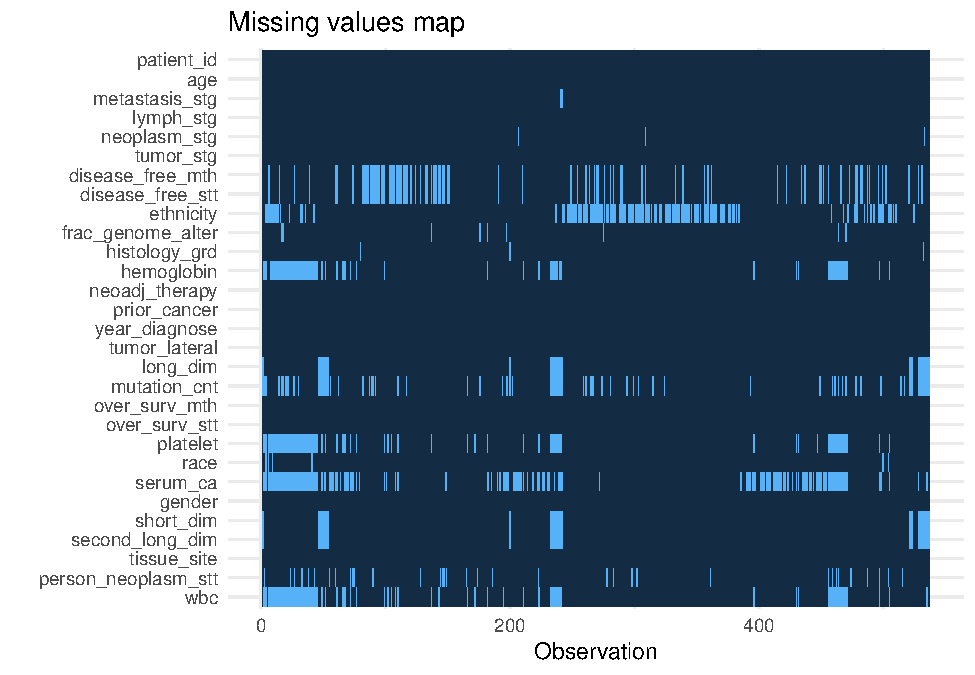
\includegraphics{figs/render-unnamed-chunk-13-1.pdf}

\begin{Shaded}
\begin{Highlighting}[]
\KeywordTok{missing_glimpse}\NormalTok{(kirc_clean4)}
\end{Highlighting}
\end{Shaded}

\begin{verbatim}
##                                   label var_type   n missing_n missing_percent
## patient_id                   patient_id    <chr> 537         0             0.0
## age                                 age    <int> 537         0             0.0
## metastasis_stg           metastasis_stg    <fct> 535         2             0.4
## lymph_stg                     lymph_stg    <fct> 537         0             0.0
## neoplasm_stg               neoplasm_stg    <fct> 534         3             0.6
## tumor_stg                     tumor_stg    <fct> 537         0             0.0
## disease_free_mth       disease_free_mth    <dbl> 438        99            18.4
## disease_free_stt       disease_free_stt    <fct> 438        99            18.4
## ethnicity                     ethnicity    <fct> 385       152            28.3
## frac_genome_alter     frac_genome_alter    <dbl> 528         9             1.7
## histology_grd             histology_grd    <fct> 534         3             0.6
## hemoglobin                   hemoglobin    <fct> 454        83            15.5
## neoadj_therapy           neoadj_therapy    <fct> 537         0             0.0
## prior_cancer               prior_cancer    <fct> 537         0             0.0
## year_diagnose             year_diagnose    <int> 537         0             0.0
## tumor_lateral             tumor_lateral    <fct> 537         0             0.0
## long_dim                       long_dim    <dbl> 502        35             6.5
## mutation_cnt               mutation_cnt    <dbl> 451        86            16.0
## over_surv_mth             over_surv_mth    <dbl> 537         0             0.0
## over_surv_stt             over_surv_stt    <fct> 537         0             0.0
## platelet                       platelet    <fct> 444        93            17.3
## race                               race    <fct> 530         7             1.3
## serum_ca                       serum_ca    <fct> 365       172            32.0
## gender                           gender    <fct> 537         0             0.0
## short_dim                     short_dim    <dbl> 502        35             6.5
## second_long_dim         second_long_dim    <dbl> 502        35             6.5
## tissue_site                 tissue_site    <fct> 537         0             0.0
## person_neoplasm_stt person_neoplasm_stt    <fct> 502        35             6.5
## wbc                                 wbc    <fct> 441        96            17.9
\end{verbatim}

\subsection{6. Checking numeric
variables}\label{checking-numeric-variables}

Check data distribution, plausible ranges, outliers; Thinking about
deleting outliers from dataset? Need to evaluate carefully each one!

\begin{Shaded}
\begin{Highlighting}[]
\NormalTok{kirc_clean4 }\OperatorTok
\StringTok{     }\KeywordTok{select_if}\NormalTok{(is.numeric) }\OperatorTok
\StringTok{     }\KeywordTok{summary}\NormalTok{()}
\end{Highlighting}
\end{Shaded}

\begin{verbatim}
##       age        disease_free_mth frac_genome_alter year_diagnose 
##  Min.   :26.00   Min.   :-11.79   Min.   :0.00000   Min.   :1998  
##  1st Qu.:52.00   1st Qu.: 13.43   1st Qu.:0.06295   1st Qu.:2004  
##  Median :61.00   Median : 36.20   Median :0.12065   Median :2006  
##  Mean   :60.59   Mean   : 40.24   Mean   :0.17016   Mean   :2006  
##  3rd Qu.:70.00   3rd Qu.: 60.51   3rd Qu.:0.20885   3rd Qu.:2007  
##  Max.   :90.00   Max.   :133.84   Max.   :0.94770   Max.   :2013  
##                  NA's   :99       NA's   :9                       
##     long_dim      mutation_cnt     over_surv_mth      short_dim     
##  Min.   :0.400   Min.   :   1.00   Min.   :  0.00   Min.   :0.1000  
##  1st Qu.:1.200   1st Qu.:  34.00   1st Qu.: 18.10   1st Qu.:0.2000  
##  Median :1.500   Median :  48.00   Median : 38.96   Median :0.3000  
##  Mean   :1.662   Mean   :  73.85   Mean   : 44.26   Mean   :0.3759  
##  3rd Qu.:2.000   3rd Qu.:  65.50   3rd Qu.: 63.21   3rd Qu.:0.5000  
##  Max.   :4.000   Max.   :1392.00   Max.   :149.05   Max.   :1.0000  
##  NA's   :35      NA's   :86                         NA's   :35      
##  second_long_dim 
##  Min.   :0.3000  
##  1st Qu.:0.7000  
##  Median :0.9000  
##  Mean   :0.9368  
##  3rd Qu.:1.1000  
##  Max.   :2.0000  
##  NA's   :35
\end{verbatim}

\begin{Shaded}
\begin{Highlighting}[]
\KeywordTok{ggplot}\NormalTok{(kirc_clean4, }\KeywordTok{aes}\NormalTok{(age)) }\OperatorTok{+}
\StringTok{     }\KeywordTok{geom_histogram}\NormalTok{(}\DataTypeTok{bins =} \DecValTok{20}\NormalTok{, }\DataTypeTok{alpha =} \FloatTok{0.8}\NormalTok{, }\DataTypeTok{color =} \StringTok{"red"}\NormalTok{)}
\end{Highlighting}
\end{Shaded}

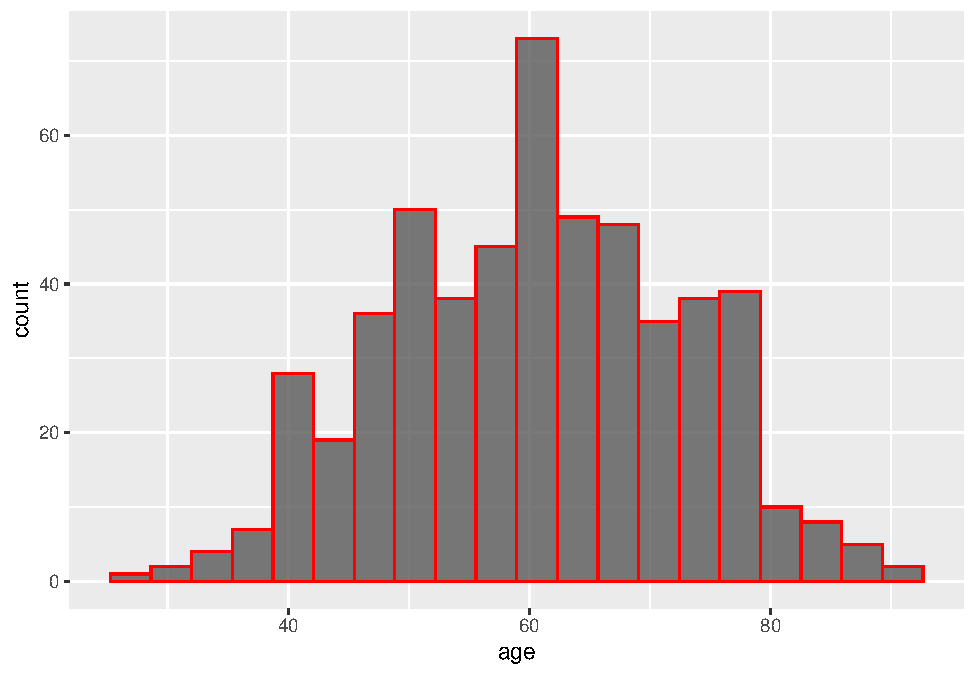
\includegraphics{figs/render-unnamed-chunk-15-1.pdf}

\begin{Shaded}
\begin{Highlighting}[]
\KeywordTok{ggplot}\NormalTok{(kirc_clean4, }\KeywordTok{aes}\NormalTok{(year_diagnose)) }\OperatorTok{+}
\StringTok{     }\KeywordTok{geom_histogram}\NormalTok{(}\DataTypeTok{bins =} \DecValTok{20}\NormalTok{, }\DataTypeTok{alpha =} \FloatTok{0.8}\NormalTok{, }\DataTypeTok{color =} \StringTok{"red"}\NormalTok{)}
\end{Highlighting}
\end{Shaded}

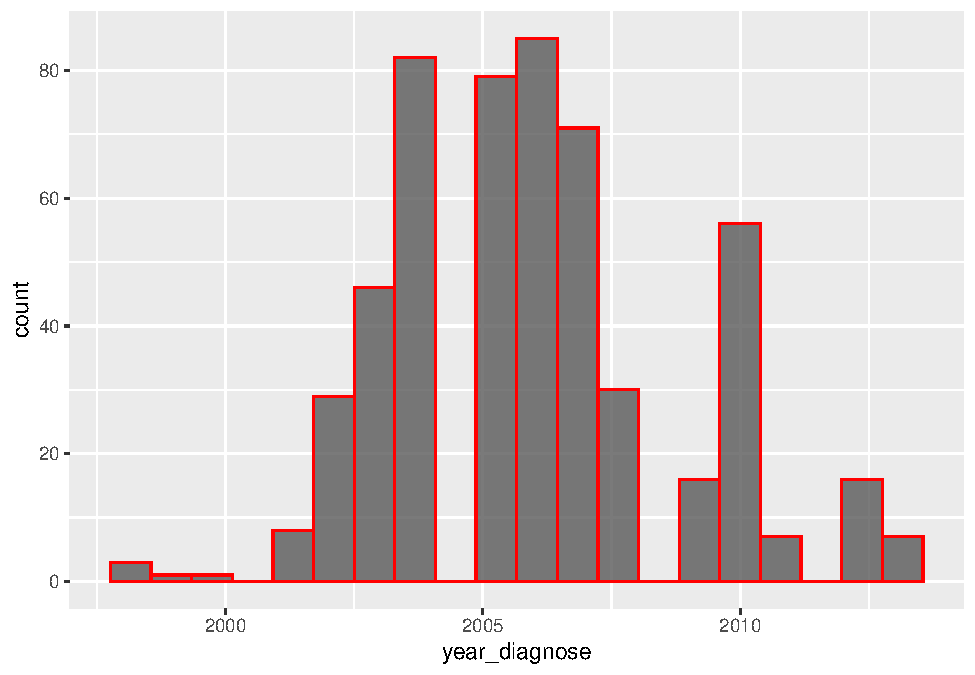
\includegraphics{figs/render-unnamed-chunk-16-1.pdf}

\begin{Shaded}
\begin{Highlighting}[]
\KeywordTok{ggplot}\NormalTok{(kirc_clean4, }\KeywordTok{aes}\NormalTok{(}\DataTypeTok{x =}\StringTok{''}\NormalTok{, }\DataTypeTok{y=}\NormalTok{disease_free_mth)) }\OperatorTok{+}
\StringTok{     }\KeywordTok{geom_boxplot}\NormalTok{(}\DataTypeTok{width =}\NormalTok{ .}\DecValTok{5}\NormalTok{) }\OperatorTok{+}
\StringTok{     }\KeywordTok{geom_jitter}\NormalTok{(}\DataTypeTok{width =} \FloatTok{0.05}\NormalTok{, }\DataTypeTok{alpha =} \FloatTok{0.2}\NormalTok{, }\DataTypeTok{color =} \StringTok{"orange"}\NormalTok{)}
\end{Highlighting}
\end{Shaded}

\begin{verbatim}
## Warning: Removed 99 rows containing non-finite values (stat_boxplot).
\end{verbatim}

\begin{verbatim}
## Warning: Removed 99 rows containing missing values (geom_point).
\end{verbatim}

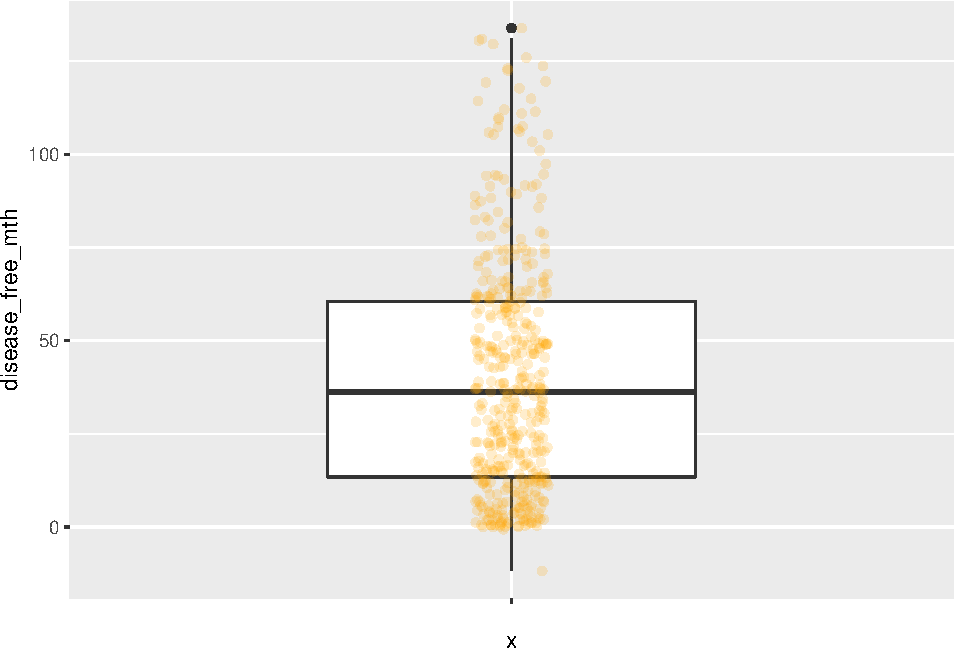
\includegraphics{figs/render-unnamed-chunk-17-1.pdf}

\begin{Shaded}
\begin{Highlighting}[]
\KeywordTok{boxplot.stats}\NormalTok{(kirc_clean4}\OperatorTok{$}\NormalTok{disease_free_mth)}
\end{Highlighting}
\end{Shaded}

\begin{verbatim}
## $stats
## [1] -11.79  13.40  36.20  60.55 130.98
## 
## $n
## [1] 438
## 
## $conf
## [1] 32.6404 39.7596
## 
## $out
## [1] 133.84
\end{verbatim}

\begin{Shaded}
\begin{Highlighting}[]
\CommentTok{# error: disease_free_mth < 0}
\end{Highlighting}
\end{Shaded}

\begin{Shaded}
\begin{Highlighting}[]
\KeywordTok{ggplot}\NormalTok{(kirc_clean4, }\KeywordTok{aes}\NormalTok{(}\DataTypeTok{x =}\StringTok{''}\NormalTok{, }\DataTypeTok{y=}\NormalTok{frac_genome_alter)) }\OperatorTok{+}
\StringTok{     }\KeywordTok{geom_boxplot}\NormalTok{(}\DataTypeTok{width =}\NormalTok{ .}\DecValTok{5}\NormalTok{) }\OperatorTok{+}
\StringTok{     }\KeywordTok{geom_jitter}\NormalTok{(}\DataTypeTok{width =} \FloatTok{0.05}\NormalTok{, }\DataTypeTok{alpha =} \FloatTok{0.2}\NormalTok{, }\DataTypeTok{color =} \StringTok{"orange"}\NormalTok{)}
\end{Highlighting}
\end{Shaded}

\begin{verbatim}
## Warning: Removed 9 rows containing non-finite values (stat_boxplot).
\end{verbatim}

\begin{verbatim}
## Warning: Removed 9 rows containing missing values (geom_point).
\end{verbatim}

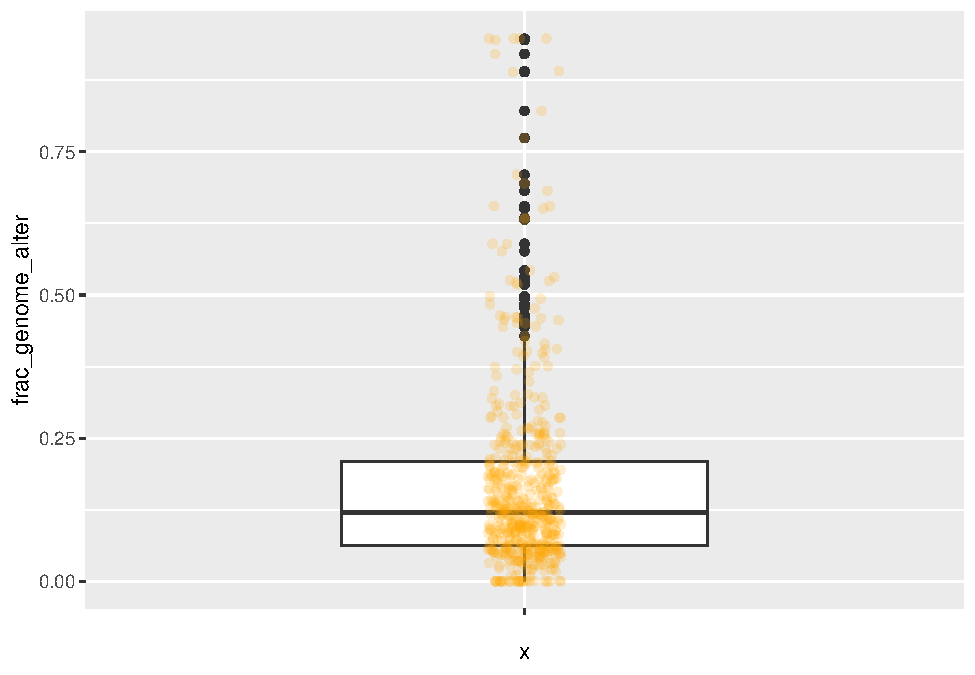
\includegraphics{figs/render-unnamed-chunk-18-1.pdf}

\begin{Shaded}
\begin{Highlighting}[]
\KeywordTok{boxplot.stats}\NormalTok{(kirc_clean4}\OperatorTok{$}\NormalTok{frac_genome_alter)}
\end{Highlighting}
\end{Shaded}

\begin{verbatim}
## $stats
## [1] 0.00000 0.06290 0.12065 0.20920 0.42800
## 
## $n
## [1] 528
## 
## $conf
## [1] 0.1105903 0.1307097
## 
## $out
##  [1] 0.8213 0.6552 0.4608 0.9477 0.5888 0.9208 0.7741 0.4837 0.9477 0.4610
## [11] 0.6549 0.6511 0.5180 0.8910 0.8893 0.9477 0.5246 0.4568 0.4937 0.9477
## [21] 0.4438 0.6947 0.5218 0.4768 0.4593 0.4447 0.9452 0.6347 0.5311 0.4562
## [31] 0.4617 0.5256 0.6318 0.5430 0.4506 0.5764 0.7102 0.4641 0.5894 0.4976
## [41] 0.4513 0.6818
\end{verbatim}

\begin{Shaded}
\begin{Highlighting}[]
\KeywordTok{ggplot}\NormalTok{(kirc_clean4, }\KeywordTok{aes}\NormalTok{(}\DataTypeTok{x =}\StringTok{''}\NormalTok{, }\DataTypeTok{y=}\NormalTok{long_dim)) }\OperatorTok{+}
\StringTok{     }\KeywordTok{geom_boxplot}\NormalTok{(}\DataTypeTok{width =}\NormalTok{ .}\DecValTok{5}\NormalTok{) }\OperatorTok{+}
\StringTok{     }\KeywordTok{geom_jitter}\NormalTok{(}\DataTypeTok{width =} \FloatTok{0.05}\NormalTok{, }\DataTypeTok{alpha =} \FloatTok{0.2}\NormalTok{, }\DataTypeTok{color =} \StringTok{"orange"}\NormalTok{)}
\end{Highlighting}
\end{Shaded}

\begin{verbatim}
## Warning: Removed 35 rows containing non-finite values (stat_boxplot).
\end{verbatim}

\begin{verbatim}
## Warning: Removed 35 rows containing missing values (geom_point).
\end{verbatim}

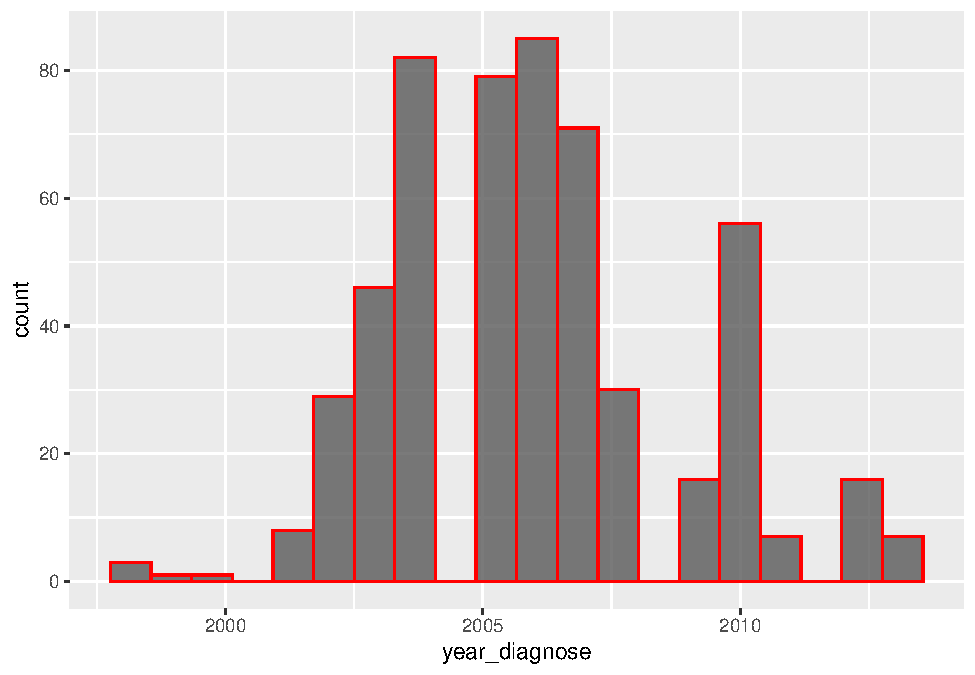
\includegraphics{figs/render-unnamed-chunk-19-1.pdf}

\begin{Shaded}
\begin{Highlighting}[]
\KeywordTok{boxplot.stats}\NormalTok{(kirc_clean4}\OperatorTok{$}\NormalTok{long_dim)}
\end{Highlighting}
\end{Shaded}

\begin{verbatim}
## $stats
## [1] 0.4 1.2 1.5 2.0 3.2
## 
## $n
## [1] 502
## 
## $conf
## [1] 1.443585 1.556415
## 
## $out
##  [1] 3.3 4.0 3.3 3.5 3.4 3.5 3.5 3.4 3.4 3.5 3.6
\end{verbatim}

\begin{Shaded}
\begin{Highlighting}[]
\KeywordTok{ggplot}\NormalTok{(kirc_clean4, }\KeywordTok{aes}\NormalTok{(}\DataTypeTok{x =}\StringTok{''}\NormalTok{, }\DataTypeTok{y=}\NormalTok{mutation_cnt)) }\OperatorTok{+}
\StringTok{     }\KeywordTok{geom_boxplot}\NormalTok{(}\DataTypeTok{width =}\NormalTok{ .}\DecValTok{5}\NormalTok{) }\OperatorTok{+}
\StringTok{     }\KeywordTok{geom_jitter}\NormalTok{(}\DataTypeTok{width =} \FloatTok{0.05}\NormalTok{, }\DataTypeTok{alpha =} \FloatTok{0.2}\NormalTok{, }\DataTypeTok{color =} \StringTok{"orange"}\NormalTok{)}
\end{Highlighting}
\end{Shaded}

\begin{verbatim}
## Warning: Removed 86 rows containing non-finite values (stat_boxplot).
\end{verbatim}

\begin{verbatim}
## Warning: Removed 86 rows containing missing values (geom_point).
\end{verbatim}

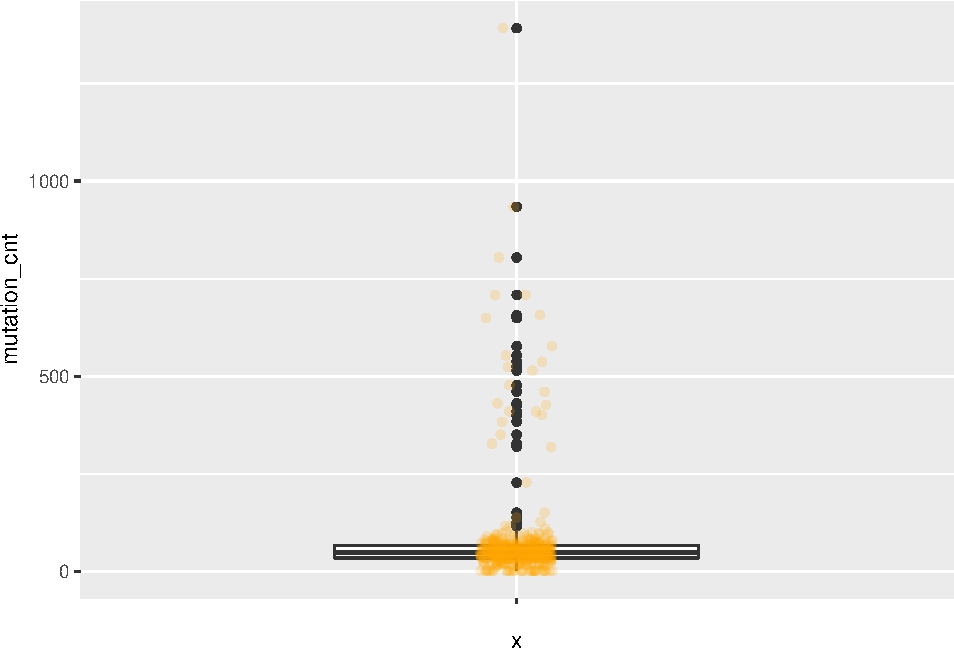
\includegraphics{figs/render-unnamed-chunk-20-1.pdf}

\begin{Shaded}
\begin{Highlighting}[]
\KeywordTok{boxplot.stats}\NormalTok{(kirc_clean4}\OperatorTok{$}\NormalTok{mutation_cnt)}
\end{Highlighting}
\end{Shaded}

\begin{verbatim}
## $stats
## [1]   1.0  34.0  48.0  65.5 109.0
## 
## $n
## [1] 451
## 
## $conf
## [1] 45.65642 50.34358
## 
## $out
##  [1]  514  656  577  537  477  150  137  708 1392  460  327  934  409  383  804
## [16]  319  524  426  227  553  400  350  410  430  708  649  126  116  115
\end{verbatim}

\begin{Shaded}
\begin{Highlighting}[]
\KeywordTok{ggplot}\NormalTok{(kirc_clean4, }\KeywordTok{aes}\NormalTok{(}\DataTypeTok{x =}\StringTok{''}\NormalTok{, }\DataTypeTok{y=}\NormalTok{over_surv_mth)) }\OperatorTok{+}
\StringTok{     }\KeywordTok{geom_boxplot}\NormalTok{(}\DataTypeTok{width =}\NormalTok{ .}\DecValTok{5}\NormalTok{) }\OperatorTok{+}
\StringTok{     }\KeywordTok{geom_jitter}\NormalTok{(}\DataTypeTok{width =} \FloatTok{0.05}\NormalTok{, }\DataTypeTok{alpha =} \FloatTok{0.2}\NormalTok{, }\DataTypeTok{color =} \StringTok{"orange"}\NormalTok{)}
\end{Highlighting}
\end{Shaded}

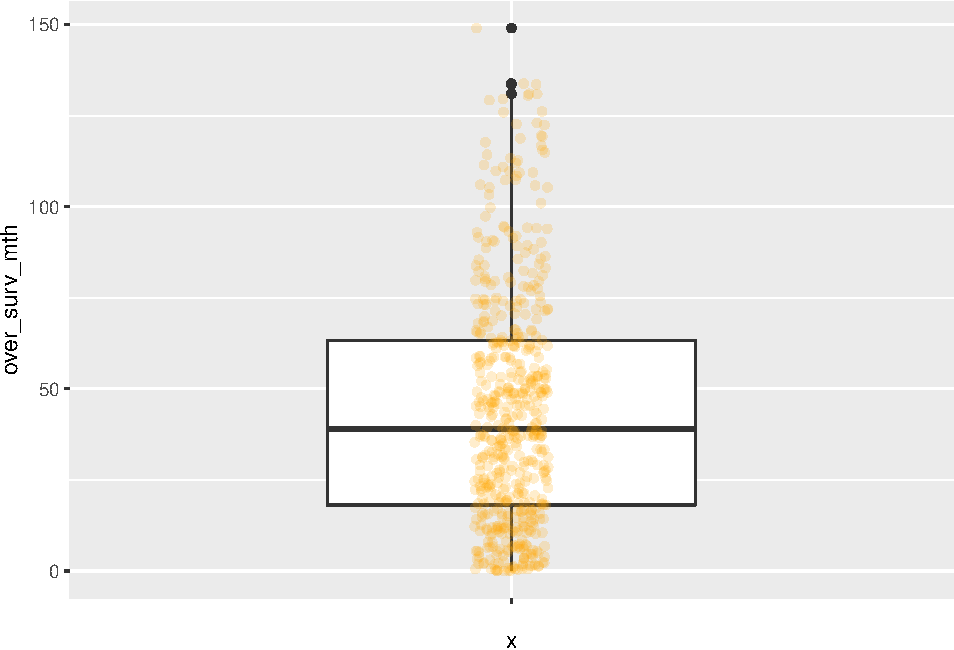
\includegraphics{figs/render-unnamed-chunk-21-1.pdf}

\begin{Shaded}
\begin{Highlighting}[]
\KeywordTok{boxplot.stats}\NormalTok{(kirc_clean4}\OperatorTok{$}\NormalTok{over_surv_mth)}
\end{Highlighting}
\end{Shaded}

\begin{verbatim}
## $stats
## [1]   0.00  18.10  38.96  63.21 130.55
## 
## $n
## [1] 537
## 
## $conf
## [1] 35.88431 42.03569
## 
## $out
## [1] 133.84 149.05 131.04 130.98 133.61
\end{verbatim}

\begin{Shaded}
\begin{Highlighting}[]
\KeywordTok{ggplot}\NormalTok{(kirc_clean4, }\KeywordTok{aes}\NormalTok{(}\DataTypeTok{x =}\StringTok{''}\NormalTok{, }\DataTypeTok{y=}\NormalTok{short_dim)) }\OperatorTok{+}
\StringTok{     }\KeywordTok{geom_boxplot}\NormalTok{(}\DataTypeTok{width =}\NormalTok{ .}\DecValTok{5}\NormalTok{) }\OperatorTok{+}
\StringTok{     }\KeywordTok{geom_jitter}\NormalTok{(}\DataTypeTok{width =} \FloatTok{0.05}\NormalTok{, }\DataTypeTok{alpha =} \FloatTok{0.2}\NormalTok{, }\DataTypeTok{color =} \StringTok{"orange"}\NormalTok{)}
\end{Highlighting}
\end{Shaded}

\begin{verbatim}
## Warning: Removed 35 rows containing non-finite values (stat_boxplot).
\end{verbatim}

\begin{verbatim}
## Warning: Removed 35 rows containing missing values (geom_point).
\end{verbatim}

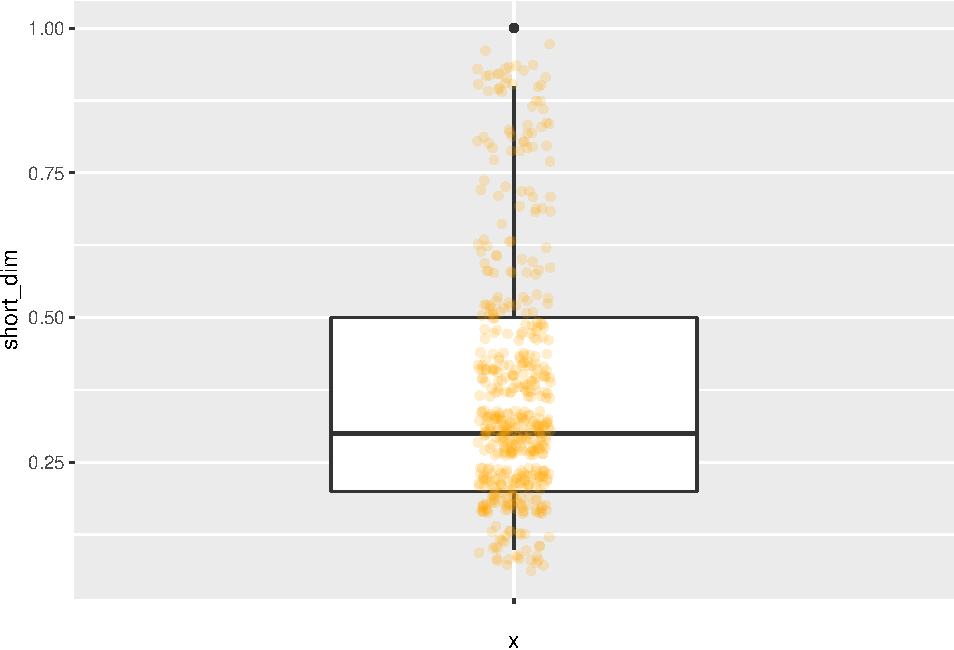
\includegraphics{figs/render-unnamed-chunk-22-1.pdf}

\begin{Shaded}
\begin{Highlighting}[]
\KeywordTok{boxplot.stats}\NormalTok{(kirc_clean4}\OperatorTok{$}\NormalTok{short_dim)}
\end{Highlighting}
\end{Shaded}

\begin{verbatim}
## $stats
## [1] 0.1 0.2 0.3 0.5 0.9
## 
## $n
## [1] 502
## 
## $conf
## [1] 0.2788443 0.3211557
## 
## $out
## [1] 1 1
\end{verbatim}

\begin{Shaded}
\begin{Highlighting}[]
\KeywordTok{ggplot}\NormalTok{(kirc_clean4, }\KeywordTok{aes}\NormalTok{(}\DataTypeTok{x =}\StringTok{''}\NormalTok{, }\DataTypeTok{y=}\NormalTok{second_long_dim)) }\OperatorTok{+}
\StringTok{     }\KeywordTok{geom_boxplot}\NormalTok{(}\DataTypeTok{width =}\NormalTok{ .}\DecValTok{5}\NormalTok{) }\OperatorTok{+}
\StringTok{     }\KeywordTok{geom_jitter}\NormalTok{(}\DataTypeTok{width =} \FloatTok{0.05}\NormalTok{, }\DataTypeTok{alpha =} \FloatTok{0.2}\NormalTok{, }\DataTypeTok{color =} \StringTok{"orange"}\NormalTok{)}
\end{Highlighting}
\end{Shaded}

\begin{verbatim}
## Warning: Removed 35 rows containing non-finite values (stat_boxplot).
\end{verbatim}

\begin{verbatim}
## Warning: Removed 35 rows containing missing values (geom_point).
\end{verbatim}

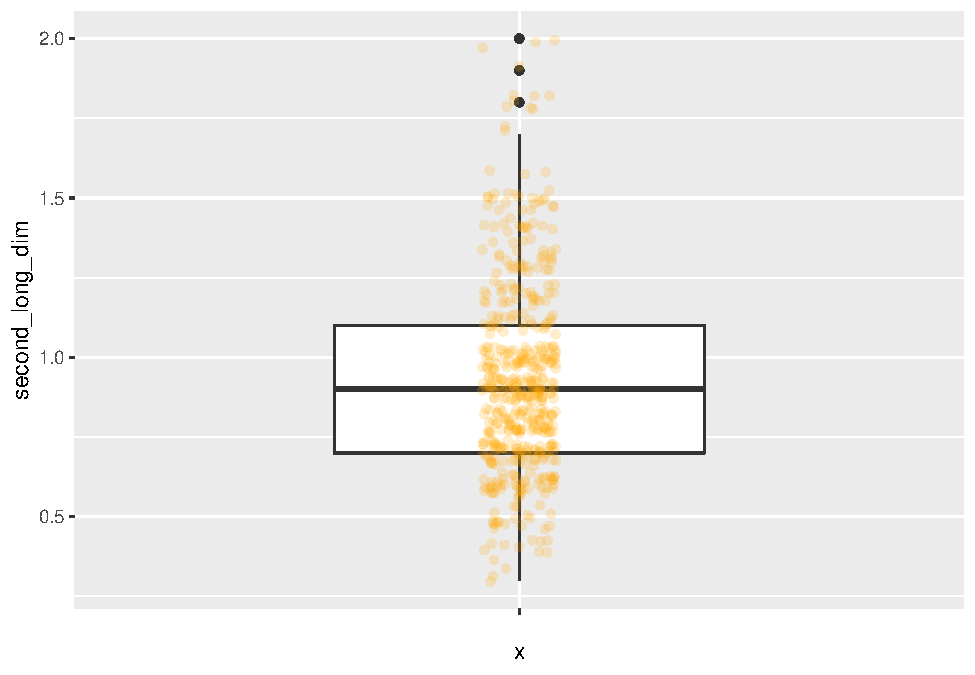
\includegraphics{figs/render-unnamed-chunk-23-1.pdf}

\begin{Shaded}
\begin{Highlighting}[]
\KeywordTok{boxplot.stats}\NormalTok{(kirc_clean4}\OperatorTok{$}\NormalTok{second_long_dim)}
\end{Highlighting}
\end{Shaded}

\begin{verbatim}
## $stats
## [1] 0.3 0.7 0.9 1.1 1.7
## 
## $n
## [1] 502
## 
## $conf
## [1] 0.8717925 0.9282075
## 
## $out
##  [1] 1.8 2.0 1.8 1.9 1.8 2.0 2.0 1.8 1.8 1.8 1.8
\end{verbatim}

\subsection{7. Checking categorical
variables}\label{checking-categorical-variables}

Check frequency, lables and levels

\begin{Shaded}
\begin{Highlighting}[]
\NormalTok{kirc_clean4 }\OperatorTok
\StringTok{     }\KeywordTok{select_if}\NormalTok{(is.factor) }\OperatorTok
\StringTok{     }\KeywordTok{summary}\NormalTok{() }
\end{Highlighting}
\end{Shaded}

\begin{verbatim}
##  metastasis_stg lymph_stg    neoplasm_stg   tumor_stg  
##  M0  :426       N0:240    Stage I  :269   T1a    :142  
##  M1  : 79       N1: 17    Stage II : 57   T3a    :122  
##  MX  : 30       NX:280    Stage III:125   T1b    :111  
##  NA's:  2                 Stage IV : 83   T2     : 55  
##                           NA's     :  3   T3b    : 53  
##                                           T1     : 22  
##                                           (Other): 32  
##             disease_free_stt                  ethnicity   histology_grd
##  DiseaseFree        :311     HISPANIC OR LATINO    : 26   G1  : 14     
##  Recurred/Progressed:127     NOT HISPANIC OR LATINO:359   G2  :230     
##  NA's               : 99     NA's                  :152   G3  :207     
##                                                           G4  : 78     
##                                                           GX  :  5     
##                                                           NA's:  3     
##                                                                        
##     hemoglobin  neoadj_therapy
##  Elevated:  5   No :519       
##  Low     :263   Yes: 18       
##  Normal  :186                 
##  NA's    : 83                 
##                               
##                               
##                               
##                                            prior_cancer   tumor_lateral
##  No                                              :459   Bilateral:  1  
##  Yes                                             : 72   Left     :253  
##  Yes, History of Prior Malignancy                :  2   Right    :283  
##  Yes, History of Synchronous/Bilateral Malignancy:  4                  
##                                                                        
##                                                                        
##                                                                        
##   over_surv_stt     platelet                          race         serum_ca  
##  DECEASED:177   Elevated: 38   ASIAN                    :  8   Elevated: 10  
##  LIVING  :360   Low     : 46   BLACK OR AFRICAN AMERICAN: 56   Low     :204  
##                 Normal  :360   WHITE                    :466   Normal  :151  
##                 NA's    : 93   NA's                     :  7   NA's    :172  
##                                                                              
##                                                                              
##                                                                              
##     gender     tissue_site  person_neoplasm_stt       wbc     
##  Female:191   BP     :142   TUMOR FREE:361      Elevated:164  
##  Male  :345   B0     :107   WITH TUMOR:141      Low     :  9  
##  MALE  :  1   CJ     : 71   NA's      : 35      Normal  :268  
##               A3     : 52                       NA's    : 96  
##               CZ     : 40                                     
##               B8     : 33                                     
##               (Other): 92
\end{verbatim}

\begin{Shaded}
\begin{Highlighting}[]
\CommentTok{# agregating levels}
\NormalTok{kirc_clin <-}\StringTok{ }\NormalTok{kirc_clean4 }\OperatorTok
\StringTok{     }\KeywordTok{mutate}\NormalTok{(}\DataTypeTok{tumor_stg =} \KeywordTok{fct_collapse}\NormalTok{(tumor_stg,}
                             \DataTypeTok{T1 =} \KeywordTok{c}\NormalTok{(}\StringTok{'T1'}\NormalTok{, }\StringTok{'T1a'}\NormalTok{, }\StringTok{'T1b'}\NormalTok{),}
                             \DataTypeTok{T2 =} \KeywordTok{c}\NormalTok{(}\StringTok{'T2'}\NormalTok{, }\StringTok{'T2a'}\NormalTok{, }\StringTok{'T2b'}\NormalTok{),}
                             \DataTypeTok{T3 =} \KeywordTok{c}\NormalTok{(}\StringTok{'T3'}\NormalTok{, }\StringTok{'T3a'}\NormalTok{, }\StringTok{'T3b'}\NormalTok{, }\StringTok{'T3c'}\NormalTok{)))}

\NormalTok{kirc_clin <-}\StringTok{ }\NormalTok{kirc_clin }\OperatorTok
\StringTok{     }\KeywordTok{mutate}\NormalTok{(}\DataTypeTok{prior_cancer =} \KeywordTok{fct_collapse}\NormalTok{(prior_cancer, }
               \DataTypeTok{Yes =} \KeywordTok{c}\NormalTok{(}\StringTok{'Yes'}\NormalTok{, }\StringTok{'Yes, History of Prior Malignancy'}\NormalTok{, }\StringTok{'Yes, History of Synchronous/Bilateral Malignancy'}\NormalTok{)))}

\NormalTok{kirc_clin <-}\StringTok{ }\NormalTok{kirc_clin }\OperatorTok
\StringTok{     }\KeywordTok{mutate}\NormalTok{(}\DataTypeTok{gender =} \KeywordTok{fct_collapse}\NormalTok{(gender, }\DataTypeTok{Male =} \KeywordTok{c}\NormalTok{(}\StringTok{'MALE'}\NormalTok{, }\StringTok{'Male'}\NormalTok{)))}
                                        
\NormalTok{kirc_clin <-}\StringTok{ }\NormalTok{kirc_clin }\OperatorTok
\StringTok{     }\KeywordTok{mutate}\NormalTok{(}\DataTypeTok{tissue_site =} \KeywordTok{fct_collapse}\NormalTok{(tissue_site,}
                         \DataTypeTok{A =} \KeywordTok{c}\NormalTok{(}\StringTok{'A3'}\NormalTok{, }\StringTok{'AK'}\NormalTok{, }\StringTok{'AS'}\NormalTok{),}
                         \DataTypeTok{B =} \KeywordTok{c}\NormalTok{(}\StringTok{'B0'}\NormalTok{, }\StringTok{'B2'}\NormalTok{, }\StringTok{'B4'}\NormalTok{, }\StringTok{'B8'}\NormalTok{, }\StringTok{'BP'}\NormalTok{),}
                         \DataTypeTok{C =} \KeywordTok{c}\NormalTok{(}\StringTok{'CJ'}\NormalTok{, }\StringTok{'CW'}\NormalTok{, }\StringTok{'CZ'}\NormalTok{),}
                         \DataTypeTok{OTHERS =} \KeywordTok{c}\NormalTok{(}\StringTok{'G6'}\NormalTok{, }\StringTok{'GK'}\NormalTok{, }\StringTok{'MM'}\NormalTok{, }\StringTok{'MW'}\NormalTok{,}
                                    \StringTok{'3Z'}\NormalTok{, }\StringTok{'6D'}\NormalTok{, }\StringTok{'DV'}\NormalTok{, }\StringTok{'EU'}\NormalTok{, }\StringTok{'T7'}\NormalTok{)))}

\CommentTok{# changing level names}
\NormalTok{kirc_clin <-}\StringTok{ }\NormalTok{kirc_clin }\OperatorTok
\StringTok{     }\KeywordTok{mutate}\NormalTok{(}\DataTypeTok{ethnicity =} \KeywordTok{fct_recode}\NormalTok{(ethnicity, }\StringTok{'hispanic/latino'}\NormalTok{=}\StringTok{'HISPANIC OR LATINO'}\NormalTok{, }\StringTok{'not hispanic/latino'}\NormalTok{=}\StringTok{'NOT HISPANIC OR LATINO'}\NormalTok{),}
            \DataTypeTok{race =} \KeywordTok{fct_recode}\NormalTok{(race, }\DataTypeTok{Asian=}\StringTok{'ASIAN'}\NormalTok{, }\StringTok{'Black/African.american'}\NormalTok{=}\StringTok{'BLACK OR AFRICAN AMERICAN'}\NormalTok{, }\DataTypeTok{White=}\StringTok{'WHITE'}\NormalTok{),}
            \DataTypeTok{person_neoplasm_stt =} \KeywordTok{fct_recode}\NormalTok{(person_neoplasm_stt, }\DataTypeTok{Tumor.Free=}\StringTok{'TUMOR FREE'}\NormalTok{, }\DataTypeTok{With.Tumor=}\StringTok{'WITH TUMOR'}\NormalTok{))}


\NormalTok{kirc_clin }\OperatorTok
\StringTok{     }\KeywordTok{select_if}\NormalTok{(is.factor) }\OperatorTok
\StringTok{     }\KeywordTok{summary}\NormalTok{()}
\end{Highlighting}
\end{Shaded}

\begin{verbatim}
##  metastasis_stg lymph_stg    neoplasm_stg tumor_stg            disease_free_stt
##  M0  :426       N0:240    Stage I  :269   T1:275    DiseaseFree        :311    
##  M1  : 79       N1: 17    Stage II : 57   T2: 69    Recurred/Progressed:127    
##  MX  : 30       NX:280    Stage III:125   T3:182    NA's               : 99    
##  NA's:  2                 Stage IV : 83   T4: 11                               
##                           NA's     :  3                                        
##                                                                                
##                ethnicity   histology_grd    hemoglobin  neoadj_therapy
##  hispanic/latino    : 26   G1  : 14      Elevated:  5   No :519       
##  not hispanic/latino:359   G2  :230      Low     :263   Yes: 18       
##  NA's               :152   G3  :207      Normal  :186                 
##                            G4  : 78      NA's    : 83                 
##                            GX  :  5                                   
##                            NA's:  3                                   
##  prior_cancer   tumor_lateral  over_surv_stt     platelet  
##  No :459      Bilateral:  1   DECEASED:177   Elevated: 38  
##  Yes: 78      Left     :253   LIVING  :360   Low     : 46  
##               Right    :283                  Normal  :360  
##                                              NA's    : 93  
##                                                            
##                                                            
##                      race         serum_ca      gender    tissue_site 
##  Asian                 :  8   Elevated: 10   Female:191   OTHERS: 28  
##  Black/African.american: 56   Low     :204   Male  :346   A     : 79  
##  White                 :466   Normal  :151                B     :303  
##  NA's                  :  7   NA's    :172                C     :127  
##                                                                       
##                                                                       
##  person_neoplasm_stt       wbc     
##  Tumor.Free:361      Elevated:164  
##  With.Tumor:141      Low     :  9  
##  NA's      : 35      Normal  :268  
##                      NA's    : 96  
##                                    
## 
\end{verbatim}

\subsection{8. Correcting and checking
again}\label{correcting-and-checking-again}

\begin{Shaded}
\begin{Highlighting}[]
\CommentTok{# month values < 0}
\NormalTok{kirc_clin}\OperatorTok{$}\NormalTok{disease_free_mth[kirc_clin}\OperatorTok{$}\NormalTok{disease_free_mth }\OperatorTok{==}\StringTok{ }\OperatorTok{-}\FloatTok{11.79}\NormalTok{] <-}\StringTok{ }\FloatTok{11.79}
\NormalTok{kirc_clin}\OperatorTok{$}\NormalTok{disease_free_mth[kirc_clin}\OperatorTok{$}\NormalTok{disease_free_mth }\OperatorTok{==}\StringTok{ }\OperatorTok{-}\FloatTok{0.62}\NormalTok{] <-}\StringTok{ }\FloatTok{0.62}

\KeywordTok{skim}\NormalTok{(kirc_clin)}
\end{Highlighting}
\end{Shaded}

\begin{longtable}[]{@{}ll@{}}
\caption{Data summary}\tabularnewline
\toprule
Name & kirc\_clin\tabularnewline
Number of rows & 537\tabularnewline
Number of columns & 29\tabularnewline
\_\_\_\_\_\_\_\_\_\_\_\_\_\_\_\_\_\_\_\_\_\_\_ &\tabularnewline
Column type frequency: &\tabularnewline
character & 1\tabularnewline
factor & 19\tabularnewline
numeric & 9\tabularnewline
\_\_\_\_\_\_\_\_\_\_\_\_\_\_\_\_\_\_\_\_\_\_\_\_ &\tabularnewline
Group variables & None\tabularnewline
\bottomrule
\end{longtable}

\textbf{Variable type: character}

\begin{longtable}[]{@{}lrrrrrrr@{}}
\toprule
skim\_variable & n\_missing & complete\_rate & min & max & empty &
n\_unique & whitespace\tabularnewline
\midrule
\endhead
patient\_id & 0 & 1 & 12 & 12 & 0 & 537 & 0\tabularnewline
\bottomrule
\end{longtable}

\textbf{Variable type: factor}

\begin{longtable}[]{@{}lrrlrl@{}}
\toprule
skim\_variable & n\_missing & complete\_rate & ordered & n\_unique &
top\_counts\tabularnewline
\midrule
\endhead
metastasis\_stg & 2 & 1.00 & FALSE & 3 & M0: 426, M1: 79, MX:
30\tabularnewline
lymph\_stg & 0 & 1.00 & FALSE & 3 & NX: 280, N0: 240, N1:
17\tabularnewline
neoplasm\_stg & 3 & 0.99 & FALSE & 4 & Sta: 269, Sta: 125, Sta: 83, Sta:
57\tabularnewline
tumor\_stg & 0 & 1.00 & FALSE & 4 & T1: 275, T3: 182, T2: 69, T4:
11\tabularnewline
disease\_free\_stt & 99 & 0.82 & FALSE & 2 & Dis: 311, Rec:
127\tabularnewline
ethnicity & 152 & 0.72 & FALSE & 2 & not: 359, his: 26\tabularnewline
histology\_grd & 3 & 0.99 & FALSE & 5 & G2: 230, G3: 207, G4: 78, G1:
14\tabularnewline
hemoglobin & 83 & 0.85 & FALSE & 3 & Low: 263, Nor: 186, Ele:
5\tabularnewline
neoadj\_therapy & 0 & 1.00 & FALSE & 2 & No: 519, Yes: 18\tabularnewline
prior\_cancer & 0 & 1.00 & FALSE & 2 & No: 459, Yes: 78\tabularnewline
tumor\_lateral & 0 & 1.00 & FALSE & 3 & Rig: 283, Lef: 253, Bil:
1\tabularnewline
over\_surv\_stt & 0 & 1.00 & FALSE & 2 & LIV: 360, DEC:
177\tabularnewline
platelet & 93 & 0.83 & FALSE & 3 & Nor: 360, Low: 46, Ele:
38\tabularnewline
race & 7 & 0.99 & FALSE & 3 & Whi: 466, Bla: 56, Asi: 8\tabularnewline
serum\_ca & 172 & 0.68 & FALSE & 3 & Low: 204, Nor: 151, Ele:
10\tabularnewline
gender & 0 & 1.00 & FALSE & 2 & Mal: 346, Fem: 191\tabularnewline
tissue\_site & 0 & 1.00 & FALSE & 4 & B: 303, C: 127, A: 79, OTH:
28\tabularnewline
person\_neoplasm\_stt & 35 & 0.93 & FALSE & 2 & Tum: 361, Wit:
141\tabularnewline
wbc & 96 & 0.82 & FALSE & 3 & Nor: 268, Ele: 164, Low: 9\tabularnewline
\bottomrule
\end{longtable}

\textbf{Variable type: numeric}

\begin{longtable}[]{@{}lrrrrrrrrrl@{}}
\toprule
skim\_variable & n\_missing & complete\_rate & mean & sd & p0 & p25 &
p50 & p75 & p100 & hist\tabularnewline
\midrule
\endhead
age & 0 & 1.00 & 60.59 & 12.15 & 26.0 & 52.00 & 61.00 & 70.00 & 90.00 &
▁▅▇▆▂\tabularnewline
disease\_free\_mth & 99 & 0.82 & 40.30 & 31.58 & 0.0 & 13.43 & 36.20 &
60.51 & 133.84 & ▇▅▃▁▁\tabularnewline
frac\_genome\_alter & 9 & 0.98 & 0.17 & 0.17 & 0.0 & 0.06 & 0.12 & 0.21
& 0.95 & ▇▂▁▁▁\tabularnewline
year\_diagnose & 0 & 1.00 & 2006.02 & 2.76 & 1998.0 & 2004.00 & 2006.00
& 2007.00 & 2013.00 & ▁▆▇▃▁\tabularnewline
long\_dim & 35 & 0.93 & 1.66 & 0.66 & 0.4 & 1.20 & 1.50 & 2.00 & 4.00 &
▃▇▃▂▁\tabularnewline
mutation\_cnt & 86 & 0.84 & 73.85 & 127.76 & 1.0 & 34.00 & 48.00 & 65.50
& 1392.00 & ▇▁▁▁▁\tabularnewline
over\_surv\_mth & 0 & 1.00 & 44.26 & 32.25 & 0.0 & 18.10 & 38.96 & 63.21
& 149.05 & ▇▇▃▂▁\tabularnewline
short\_dim & 35 & 0.93 & 0.38 & 0.21 & 0.1 & 0.20 & 0.30 & 0.50 & 1.00 &
▆▇▂▁▁\tabularnewline
second\_long\_dim & 35 & 0.93 & 0.94 & 0.31 & 0.3 & 0.70 & 0.90 & 1.10 &
2.00 & ▃▇▆▂▁\tabularnewline
\bottomrule
\end{longtable}

\subsection{9. Saving dataset}\label{saving-dataset}

\begin{Shaded}
\begin{Highlighting}[]
\KeywordTok{write_csv}\NormalTok{(kirc_clin, }\DataTypeTok{path =} \StringTok{"data/kirc_clin.csv"}\NormalTok{)}

\KeywordTok{rm}\NormalTok{(kirc_clean4, kirc_clean3, kirc_clean2, kirc_clean1, kirc_clean0, kirc_clean, NA_sum, NA_fifty)}
\end{Highlighting}
\end{Shaded}

\subsection{Further analysis}\label{further-analysis}

\begin{itemize}
\tightlist
\item
  \href{2.correlation.md}{Comparison and Hyphotesis test}
\item
  \href{3.logistic_regression.md}{Logistic Regression Model}
\end{itemize}

\begin{Shaded}
\begin{Highlighting}[]
\KeywordTok{sessionInfo}\NormalTok{()}
\end{Highlighting}
\end{Shaded}

\begin{verbatim}
## R version 3.6.3 (2020-02-29)
## Platform: x86_64-apple-darwin15.6.0 (64-bit)
## Running under: macOS Mojave 10.14.6
## 
## Matrix products: default
## BLAS:   /Library/Frameworks/R.framework/Versions/3.6/Resources/lib/libRblas.0.dylib
## LAPACK: /Library/Frameworks/R.framework/Versions/3.6/Resources/lib/libRlapack.dylib
## 
## locale:
## [1] pt_BR.UTF-8/pt_BR.UTF-8/pt_BR.UTF-8/C/pt_BR.UTF-8/pt_BR.UTF-8
## 
## attached base packages:
## [1] stats     graphics  grDevices utils     datasets  methods   base     
## 
## other attached packages:
##  [1] finalfit_1.0.2  skimr_2.1.1     forcats_0.5.0   stringr_1.4.0  
##  [5] dplyr_0.8.5     purrr_0.3.3     readr_1.3.1     tidyr_1.0.2    
##  [9] tibble_3.0.0    ggplot2_3.3.0   tidyverse_1.3.0
## 
## loaded via a namespace (and not attached):
##  [1] Rcpp_1.0.4       lubridate_1.7.8  lattice_0.20-41  assertthat_0.2.1
##  [5] digest_0.6.25    utf8_1.1.4       R6_2.4.1         cellranger_1.1.0
##  [9] repr_1.1.0       backports_1.1.6  reprex_0.3.0     evaluate_0.14   
## [13] highr_0.8        httr_1.4.1       pillar_1.4.3     rlang_0.4.5     
## [17] readxl_1.3.1     rstudioapi_0.11  Matrix_1.2-18    rmarkdown_2.1   
## [21] labeling_0.3     splines_3.6.3    munsell_0.5.0    broom_0.7.0     
## [25] compiler_3.6.3   modelr_0.1.6     xfun_0.12        pkgconfig_2.0.3 
## [29] base64enc_0.1-3  htmltools_0.4.0  tidyselect_1.0.0 fansi_0.4.1     
## [33] crayon_1.3.4     dbplyr_1.4.2     withr_2.1.2      grid_3.6.3      
## [37] jsonlite_1.6.1   gtable_0.3.0     lifecycle_0.2.0  DBI_1.1.0       
## [41] magrittr_1.5     scales_1.1.0     cli_2.0.2        stringi_1.4.6   
## [45] farver_2.0.3     fs_1.4.1         mice_3.8.0       xml2_1.3.0      
## [49] ellipsis_0.3.0   generics_0.0.2   vctrs_0.2.4      boot_1.3-24     
## [53] tools_3.6.3      glue_1.4.0       hms_0.5.3        survival_3.2-3  
## [57] yaml_2.2.1       colorspace_1.4-1 rvest_0.3.5      knitr_1.28      
## [61] haven_2.2.0
\end{verbatim}

\end{document}
